\chapter{Approccio terapeutico al linfoma non Hodgkin}

\section{"Watch and wait"}
L’approccio terapeutico al linfoma non-Hodgkin, dipende da diversi fattori: dal sottotipo di linfoma, 
dallo stadio della malattia, dall’eventuale presenza di “sintomi B” come febbre, sudorazione notturna, 
perdita di peso superiore al 10\% negli ultimi sei mesi, ed il possibile coinvolgimento extranodale\cite{LLS}.\\
L’approccio “watch and wait” viene scelto per pazienti con linfoma indolente, che non presentano sintomi e che 
alla diagnosi mostrano un’estensione della patologia limitata. 
Si tratta di un’osservazione attenta nel corso del tempo, mediante analisi ed esami mirati.\\
Alcuni studi hanno mostrato come non ci fosse una differenza a livello di sopravvivenza tra i pazienti che venivano 
fin da subito sottoposti a trattamento rispetto a chi invece veniva osservato nel tempo; l’approccio da scegliere 
viene concordato tra il medico e il paziente, in quanto ogni caso è a sé e deve essere valutato singolarmente\cite{LLS}.\\
Per alcuni pazienti la malattia può restare stabile o progredire lentamente per molti anni, 
per altri invece può evolvere in forme aggressive di LNH che necessita pertanto di trattamento tempestivo.\\
Per pazienti con linfoma aggressivo invece si ha un approccio di polichemioterapia basata su schemi terapeutici 
che associano farmaci chemioterapici, corticosteroidi e anticorpi monoclonali. 
Per quel che riguarda la chemioterapia, sarà approfondita in un capitolo a parte.\\ 
In questo capitolo ci concentreremo su altri approcci terapeutici: 
radioterapia, immunoterapia, trapianto autologo e allogenico di cellule staminali emopoietiche.\\

\section{Radioterapia}
La radioterapia usa radiazioni ad alte dosi per distruggere le cellule cancerose o per rallentare la loro crescita, 
distruggendo il loro DNA. 
La radioterapia può essere esterna o interna, quest'ultima è detta anche brachiterapia. 
La caratteristica della radioterapia esterna è che è un trattamento localizzato, cioè rivolto alla sola parte 
del corpo interessata dal tumore. 
Per quanto riguarda la radioterapia interna, possiamo parlare di brachiterapia o di radioterapia sistemica. 
La brachiterapia è un trattamento locale, quindi di una specifica parte del corpo, in cui particelle contenenti 
radiazioni vengono immesse nel tumore o nelle sue vicinanze. 
La radioterapia sistemica è così definita perché il trattamento è immesso nel corpo per via orale, endovenosa o 
tramite iniezione e questo modo raggiunge tutti i tessuti del corpo; con questo trattamento i liquidi biologici 
come urina, saliva e sudore, risulteranno radioattivi per qualche giorno, fino a che il corpo non avrà smaltito 
tali sostanze\cite{NIH}.\\
Nel LNH, la radioterapia è usata come unico trattamento in caso di stadi di malattia molto precoci, 
altrimenti è un trattamento generalmente combinato ad altri, come la chemioterapia, nonché può essere 
coadiuvata al trapianto di cellule staminali; può essere anche impiegata per alleviare i sintomi causati da 
linfomi che interessano cervello, midollo spinale e per tumori che comprimono i nervi\cite{ACSRADIATION}.\\
È impiegata in caso di malattia bulky o dopo il trattamento di chemioterapia per prevenire le recidive. 
Prima della radioterapia il team deve pianificare il trattamento: decide la dose necessaria, bisogna assicurarsi 
che il trattamento sia rivolto principalmente alle cellule cancerose e il meno possibile alle cellule sane, 
per evitare di danneggiarle; si esegue una TC dell’area da trattare, un momento in cui è di fondamentale importanza 
mantenere una posizione ferma, in quanto essa viene registrata e sarà la posizione in cui verrà eseguita la 
radioterapia\cite{MACMILLAN}.\\
In caso di radioterapia che interessa testa e collo vengono prodotti degli immobilizzatori che aiutano a mantenere 
la postura. La durata del trattamento dipende dal tipo e dall’estensione del linfoma, il trattamento non provoca 
dolore, si sentono i rumori emessi dalla macchina e si può comunicare con il team tramite dei microfoni, da cui 
possono dare indicazioni o a cui ci si può rivolgere in caso di malessere\cite{UKRADIOTP}.\\

\subsection{Effetti collaterali della radioterapia}
Gli effetti collaterali della radioterapia dipendono dalla parte del corpo interessata dal trattamento; 
medici e infermieri informano il paziente sulla possibilità che diversi sintomi possono presentarsi, la gravità e 
la durata del sintomo variano da persona a persona. 
Il paziente viene informato su come gestire tali sintomi, è importante informare il medico per quanto riguarda la 
loro comparsa ed avvisare se persistono o peggiorano. Effetti a lungo termine sono rari e dipendono dalla parte 
del corpo trattata\cite{MACMILLAN}.\\
La radioterapia per il LNH può provocare, nel breve termine, arrossamento e dolore della pelle, a livello dell’area 
trattata; la pelle può sembrare una scottatura solare, può dare prurito e formare vescicole; questi cambiamenti possono
presentarsi fino a 2-4 settimane dopo la fine del trattamento. Bisogna seguire alcuni accorgimenti di skin care 
dell’area trattata: non usare borotalco, quando ci si lava usare acqua e sapone senza strofinare vigorosamente, 
asciugare tamponando; non usare profumi, non eseguire ceretta; si può usare il deodorante normalmente, a meno che 
la pelle non sia danneggiata; gli uomini possono usare rasoi elettrici; non applicare medicazioni; si può eseguire 
lo shampoo, ma non asciugare i capelli con l’asciugacapelli, se il trattamento interessa la testa.\\ 
Durante il trattamento di radioterapia, indossare indumenti comodi, prodotti con fibre naturali, evitare i reggiseni; 
fare attenzione all’esposizione al sole fino ad un anno dopo la fine della radioterapia, usando sempre la crema 
solare ad alta protezione\cite{UKRADIOTP}.\\
Stanchezza, affaticamento e debolezza sono sintomi passeggeri, che aumentano con il progredire del trattamento e che 
possono permanere anche per qualche settimana dalla fine del trattamento; una strategia di coping per la stanchezza è 
di programmare delle attività da alternare poi con il riposo, è normale passare molte ore a dormire, soprattutto in 
caso di radioterapia combinata ad altri trattamenti come il trapianto di cellule staminali.\\ 
In base alla parte del corpo trattata, possono verificarsi anche diarrea, nausea e perdita dei capelli. In caso di 
diarrea, è importante restare idratati per compensare la perdita di liquidi, seguire una dieta povera di fibre e 
inoltre il medico può prescrivere dei farmaci per ridurre il numero di scariche diarroiche; questo sintomo dovrebbe 
risolversi in poche settimane dalla fine del trattamento, è importante segnalare se continua. La nausea si può 
verificare nei primi giorni dall’inizio del trattamento, in genere il medico prescrive dei farmaci per alleviare 
tale sintomatologia.\\ 
La perdita dei capelli e dei peli, può iniziare dopo qualche settimana dalla fine del trattamento, nell’area 
interessata dalla radioterapia, è anche questa una condizione temporanea, la crescita riprende quando il trattamento 
cessa\cite{UKRADIOTP}.\\ 

\section{Immunoterapia}
L’immunoterapia è un trattamento usato per il cancro e il principio su cui si basa, è di migliorare la capacità 
del sistema immunitario del corpo di individuare ed attaccare le cellule cancerose. 
Il sistema immunitario ha la funzione di riconoscere ed eliminare cellule anomale, ma alcune cellule cancerose 
riescono ad evadere dai meccanismi di difesa che vengono messi in atto, anche se il sistema immunitario è sano. 
L’immunoediting è quel processo che le cellule cancerose mettono in atto per evadere dall’immunosorveglianza del 
sistema immunitario; il processo prevede tre fasi: eliminazione, equilibrio ed evasione. Le immunoterapie vanno 
proprio a stimolare l’attivazione o la riattivazione del sistema immunitario nei confronti delle cellule cancerose 
che sono riuscite ad evadere\cite{IMMUNOTP}.\\
Per il LNH, il trattamento di immunoterapia prevede la somministrazione di anticorpi monoclonali, 
la terapia delle CAR-T, gli inibitori del checkpoint immunitario o immune checkpoint inhibitors, 
immunomodulatori o immunomodulators.\\

\subsection{Anticorpi monoclonali}
Gli anticorpi sono proteine prodotte naturalmente dal nostro corpo come risposta di difesa verso diversi tipi di 
antigeni. Gli anticorpi monoclonali sono versioni man-made, prodotte per stimolare il sistema immunitario a reagire 
nei confronti di determinate cellule; vengono definiti anche “target therapy” in quanto alcuni anticorpi monoclonali 
sono diretti in modo specifico verso alcune cellule cancerose, le devono localizzare e a cui devono attaccarsi per 
poterle colpire\cite{IMMUNOTP}.\\
Sono diversi i tipi di anticorpi monoclonali usati per il trattamento del LNH, in quanto possono avere come target 
diverse proteine. 
Alcuni anticorpi monoclonali hanno come target la proteina CD20, che si trova sulla superficie dei linfociti B. 
Esempi di tali anticorpi sono: rituximab (rituxan), obinutuzumab (Gazyva), ofatumumab (arzerra). 
Essi fanno parte degli anticorpi monoclonali definiti “naked” in quanto non sono legati ad altri farmaci o a 
molecole radioattive, ma funzionano da soli\cite{LLSIMMUNO}.\\
Altri anticorpi hanno come target la proteina CD30, presente sulla superficie dei linfociti B e T; 
ad esempio il Brentuximab vedotin (adcetris), il quale fa parte della classe degli anticorpi monoclonali coniugati, 
così definiti perché sono legati ad un farmaco chemioterapico o ad una molecola radioattiva, in questo caso 
Brentuximab è coniugato ad un farmaco chemioterapico. Di questa classe inoltre fa parte il farmaco 
Yttrium-90-ibritumomab tiuxetan (Zevalin), un esempio di radioimmunoterapia dove l’anticorpo monoclonale è coniugato 
ad un isotopo radioattivo, ed esplica la sua funzione direttamente sulle cellule tumorali; esso ha però come target 
la proteina CD20\cite{LLSIMMUNO}.\\
Infine vi sono gli anticorpi monoclonali bispecifici, costituiti da due anticorpi monoclonali che possono avere come 
target due proteine diverse contemporaneamente. Ad esempio blinatumomab (blincyto) ha come target la proteina CD19 
presente cellule cellule B, ma anche la proteina CD3, presente sulla superficie dei linfociti T\cite{LLSIMMUNO}.\\
Gli anticorpi monoclonali vengono somministrati solitamente per via endovenosa, il trattamento può durare anche 
diverse ore, e in genere vengono combinati con cicli di chemioterapia; i farmaci chemioterapici impiegati dipendono 
dallo schema terapeutico in atto per il paziente, pertanto anche l’anticorpo monoclonale viene somministrato 
seguendo dei cicli\cite{IMMUNOTP}.\\

Gli anticorpi monoclonali possono provocare degli effetti collaterali nell’immediato subito durante l’infusione o 
qualche ora dopo. 
Possono essere sintomi generici o correlati ad una reazione allergica, in tal caso si potranno manifestare brividi, 
rialzo febbrile, eruzioni cutanee, vertigini, mal di testa, mal di schiena, dispnea. 
Sintomi generici che possono manifestarsi sono anche  fatigue, debolezza, sintomi simil-influenzali, nausea, vomito, 
diarrea, dolore toracico, aumento della frequenza cardiaca\cite{LLSIMMUNO}.\\
È importante che questi sintomi vengano individuati o riferiti dal paziente in modo da poterli trattare.		
Questi farmaci inoltre possono anche causare una riattivazione del virus dell’epatite B, pertanto prima di iniziare 
il trattamento saranno eseguiti degli esami ematici specifici, per verificare l’eventuale presenza di tale virus ed 
anche diversi mesi dopo la fine del trattamento, si è esposti al rischio di sviluppare infezioni. 
L’utilizzo del brentuximab vedotin può provocare neuropatia,alterazioni  dell’ emocromo , infezioni, tosse, febbre, 
nausea, vomito, diarrea, fatigue\cite{IMMUNOTP}.\\

Tra le target therapies, per il LNH a basso grado di malignità, viene impiegato Bortezomib, nel linfoma a cellule del 
mantello che non è stato trattato prima e non si può ricorrere al trapianto di cellule staminali. Bortezomib, fa parte 
dei protesome inhibitors, infatti agisce andando a impedire la distruzione 
delle proteine all’interno delle cellule e ciò fa sì che le cellule cancerose vadano incontro a morte cellulare\cite{LYMPHOMACTION}.\\
Esso è stato approvato dall’FDA per la somministrazione per via endovenosa o sottocutanea e in genere viene associato 
ad altri farmaci chemioterapici all’interno di schemi terapeutici. L’effetto collaterale più comune per quanto 
riguarda Bortezomib è la neuropatia periferica, la quale risulta ridotta nella somministrazione sottocutanea piuttosto 
che in quella endovenosa. La via sottocutanea risulta più vantaggiosa in quanto ha un assorbimento più rapido rispetto 
alla via orale, l’assorbimento nel tessuto adiposo è prolungato nel tempo rispetto alla via intramuscolare e 
risulta una buona alternativa alla via endovenosa in caso di pazienti con scarso patrimonio venoso\cite{BORTEZOMIB}.\\
Bisogna tuttavia avere degli accorgimenti per quanto riguarda la tecnica di somministrazione, per ridurre al minimo 
le reazioni locali correlate alla somministrazione SC di chemioterapici.\\

\begin{figure}[h]
    \begin{center}
    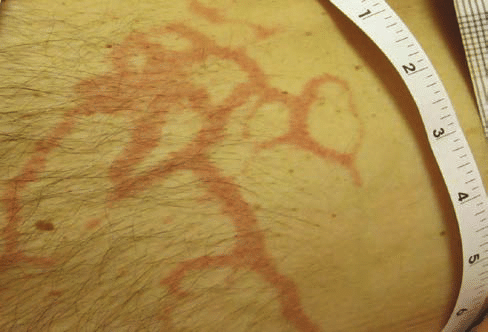
\includegraphics[width=0.8\columnwidth]{img/Atypical-reaction-to-bortezomib-with-spiderlike-extensions-of-erythema-Figure-2-Local.png}
    \end{center}
    \caption[ Reazione atipica dopo la somministrazione di Bortezomib]{ Reazione atipica dopo la somministrazione di Bortezomib
    \cite{img28}}

\end{figure}

\begin{figure}[h]
    \begin{center}
    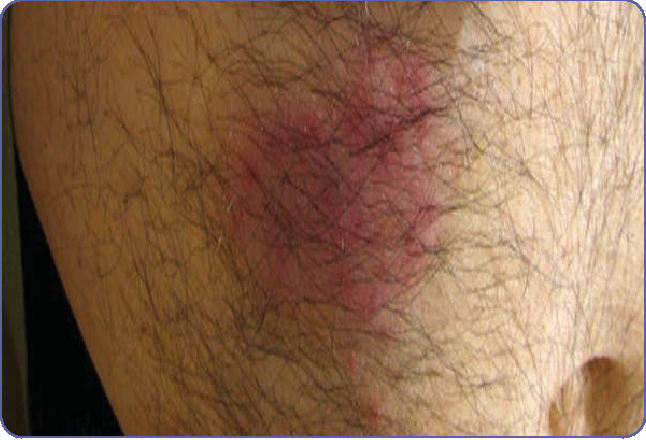
\includegraphics[width=0.6\columnwidth]{img/bort reaction.png}
    \end{center}
    \caption[ Reazione al Bortezomib dopo somministrazione per via sottocutanea]{ Reazione al Bortezomib dopo somministrazione per via sottocutanea
    \cite{img29}}

\end{figure}

\begin{figure}[h]
    \begin{center}
    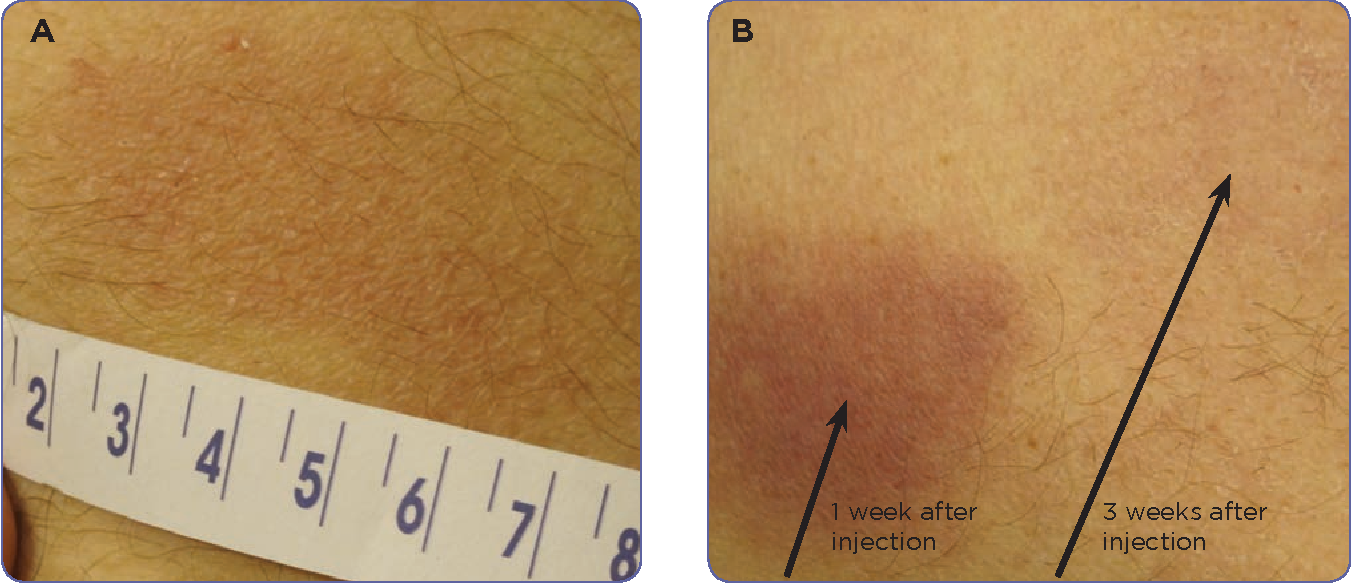
\includegraphics[width=0.8\columnwidth]{img/bortezomib reaction.png}
    \end{center}
    \caption[ Reazione al Bortezomib]{ Reazione al Bortezomib
    \cite{img30}}

\end{figure}

\begin{figure}[h]
    \begin{center}
    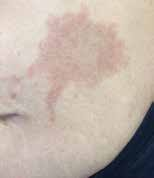
\includegraphics[width=0.5\columnwidth]{img/bortezomib reaction2.jpeg}
    \end{center}
    \caption[ Reazione avversa al Bortezomib]{ Reazione avversa al Bortezomib
    \cite{img31}}

\end{figure}

L’infermiere è responsabile della somministrazione di Bortezomib per via sottocutanea e pertanto deve osservare tutti 
gli accorgimenti necessari per ridurre al minimo la probabilità di sviluppare reazioni cutanee, attraverso una serie 
di step. Scegliere il sito di iniezione più adatto, ricordando che non ci sono evidenze che raccomandano l’iniezione 
nella regione deltoidea che, pertanto, deve essere evitata. Evitare zone in cui si evidenziano rossore, calore, 
tumefazione, noduli, cute non integra, escoriazioni, segni di infiammazione. Ruotare le sedi di iniezione, evitando 
la zona periombelicale e documentare in cartella la sede di iniezione utilizzata in modo da usarne 
un’altra per la successiva somministrazione\cite{BORTNURSES}.\\

\begin{figure}[h]
    \begin{center}
    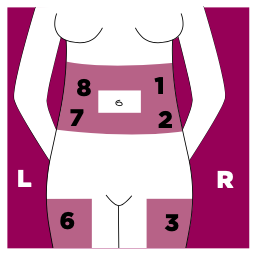
\includegraphics[width=0.5\columnwidth]{img/SEDI.png}
    \end{center}
    \caption[ Sedi di iniezione di Bortezomib per via sottocutanea]{ Sedi di iniezione di Bortezomib per via sottocutanea
    \cite{img32}}

\end{figure}

La tecnica di iniezione prevede di sollevare la plica cutanea prestando attenzione a sollevare il tessuto 
sottocutaneo ma non quello muscolare. Il volume massimo iniettabile mediante questa via è comunque di 2 mL.\\

\begin{figure}[h]
    \begin{center}
    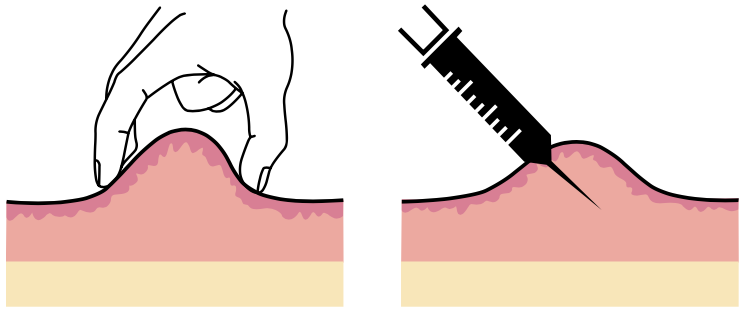
\includegraphics[width=0.8\columnwidth]{img/PLICA.png}
    \end{center}
    \caption[ Tecnica di iniezione con la plica cutanea.]{ Tecnica di iniezione con la plica cutanea.
    \cite{img33}}

\end{figure}

La scelta dell’ago appropriato è inoltre importante. Un ago da 26G è indicato per la somministrazione con un angolo di
90°, mentre se si opta per un angolo di 45° bisognerà usare un ago più piccolo per non incorrere nel rischio di 
penetrare nel tessuto muscolare\cite{BORTNURSES}.\\
Per la somministrazione di Bortezomib per via sottocutanea, risulta appropriata la tecnica air sandwich, 
da non usare invece per la via di somministrazione endovenosa. Questa tecnica, che prevede di aspirare 0.5-1 mL 
di aria nella siringa, che non deve essere rimossa, viene utilizzata per ridurre l‘irritazione da parte del farmaco e 
per garantire la somministrazione dell’intera dose. L’iniezione infine deve essere lenta, facendo delle pause, 
di circa 10 secondi. Al termine rimuovere l’ago e applicare una leggera pressione senza strofinare\cite{BORTNURSES}.\\

\begin{figure}[h]
    \begin{center}
    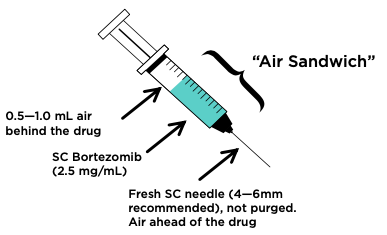
\includegraphics[width=0.8\columnwidth]{img/SIRINGA.png}
    \end{center}
    \caption[ Air sandwich technique]{ Air sandwich technique
    \cite{img34}}

\end{figure}

Reazioni sul sito di iniezione possono sempre manifestarsi, pertanto bisogna educare il paziente riguardo il 
trattamento: possono essere assunti antistaminici per via orale, l’applicazione per via topica di impacchi freddi, 
creme antistaminiche o cortisoniche sono raccomandate dopo quattro ore dall’iniezione, 
applicarle prima potrebbe provocare dei cambiamenti nella farmacocinetica\cite{BORTEZOMIB}.\\
La neuropatia periferica è il principale effetto collaterale correlato alla somministrazione di bortezomib, 
ma numerosi sono gli effetti collaterali che ne derivano: trombocitopenia, infezione, ipotensione, disturbi 
gastrointestinali, tumor lysis syndrome, problemi a livello cardiaco e polmonare, posterior reversible 
encephalopathy syndrome (PRES)\cite{BORTNURSES}.\\ 

\subsection{CAR-T (CHIMERIC ANTIGEN RECEPTOR)}

La terapia cellulare con CAR-T (chimeric antigen receptor) è una forma di terapia genica impiegata per forme 
refrattarie e recidivanti  i cui risultati più importanti si hanno per la leucemia linfoblastica acuta e per il 
linfoma non Hodgkin (LNH). Sono in corso ricerche che consentano l’impiego di tale metodica anche per altre neoplasie 
ematologiche nonché per i tumori solidi.
L’European Medicines Agency (EMA) ha dato l’approvazione commerciale di due CAR-T di seconda generazione: 
tisagenlecleucel (tisa-cel, KymriahTM, Novartis) e axicabtagene ciloleucel (axi-cel, YescartaTM, Gilead), 
che sono anche i prodotti disponibili in Italia\cite{reteveneta}.\\
La FDA (Food and Drugs Administration) ha invece approvato sei farmaci, come 
riportato dal National Cancer Institute\cite{NIHCART}.\\

\begin{figure}[h]
    \begin{center}
    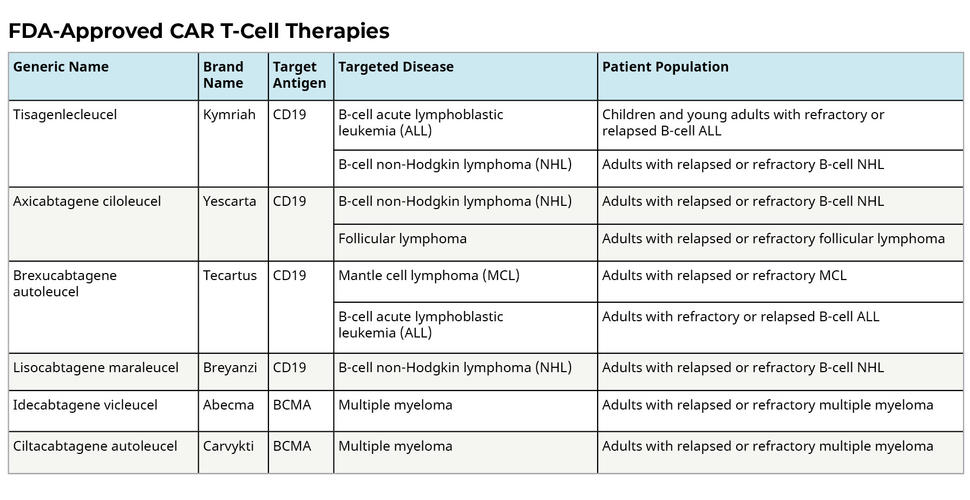
\includegraphics[width=1.0\columnwidth]{img/FDA Approved CAR T-Cell Therapies Table.jpeg}
    \end{center}
    \caption[Farmaci CAR-T approvati dall’FDA]{Farmaci CAR-T approvati dall’FDA
    \cite{img22}}

\end{figure}

Nel caso del LNH, il Tisagenlecleucel è indicato per i linfomi diffusi a grandi cellule B (DLBCL) recidivanti o 
refrattari dopo due linee di chemioterapia sistemica. L’ Axicabtageneciloleucel è stato approvato per linfomi 
diffusi a grandi cellule B (DLBCL) e linfoma a grandi cellule B primitivo del mediastino, 
refrattari o recidivanti, dopo due linee di chemioterapia sistemica\cite{EMATOCART}.\\
Il CAR è un recettore transmembrana chimerico, che, mediante l’utilizzo di vettori retrovirali o lentivirali, 
va a sostituire il TCR del linfocita.  
La terapia delle CAR-T è autologa, in quanto usa le cellule T proprie del paziente. La loro produzione sfrutta 
il processo di ingegnerizzazione.\\

La prima fase del processo di produzione delle CAR-T è la leucoaferesi, in cui viene prelevato il sangue dal 
paziente tramite una vena periferica; grazie al processo di aferesi il sangue prelevato viene separato in 
globuli rossi, globuli bianchi, piastrine e plasma, ma solo le cellule T dei globuli bianchi vengono prelevate, 
mentre il resto del sangue viene reinfuso al paziente. È una fase molto importante e delicata in quanto una bassa 
resa aferetica, provoca una ridotta espansione delle cellule CAR-T in vitro; questo può dipendere da una bassa conta 
leucocitaria, dalla presenza di numerose cellule natural killer (NK) e blasti nel sangue periferico\cite{EMATOCART},\cite{LLSCART}.\\
La seconda fase del processo prevede che le cellule T raccolte siano inviate a laboratori specializzati per la fase 
di ingegnerizzazione genetica, secondo cui il DNA viene introdotto all’interno delle cellule, per produrre CAR, 
grazie ai quali le cellule T acquisiscono la capacità di attaccare le cellule cancerose\cite{EMATOCART},\cite{LLSCART}.\\
Nella terza fase, il numero di cellule raccolte viene moltiplicato in laboratorio e quando si ha il quantitativo 
necessario, vengono criopreservate e rinviate al centro o all’ospedale dove il paziente le riceverà. 
Questo processo dura dalle tre alle quattro settimane.\\
Prima della somministrazione, il paziente, a partire da una settimana fino a due giorni prima, viene sottoposto 
alla chemioterapia di linfodeplezione che  serve a ridurre le cellule T normali nel corpo, per “fare spazio” alle 
cellule CAR-T ed avere una maggiore espansione in vivo.\\ 
Lo schema terapeutico maggiormente utilizzato prevede la somministrazione di ciclofosfamide e fludarabina.
L’ultima fase è di somministrazione del farmaco, previo scongelamento, in una via endovenosa centrale, 
della durata di circa trenta minuti\cite{EMATOCART}.\\
I centri autorizzati alla somministrazione delle CAR-T sono presenti in tutta Italia, in Toscana abbiamo 
i centri di Firenze e Pisa\cite{AILCENTRI}.\\

\begin{figure}[h]
    \begin{center}
    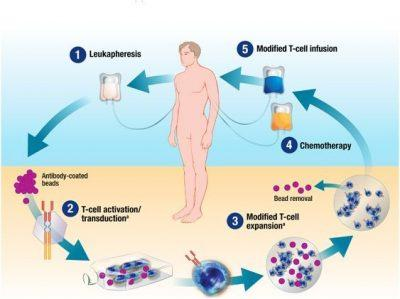
\includegraphics[width=1.0\columnwidth]{img/car-t process.jpeg}
    \end{center}
    \caption[Processo di costituzione e somministrazione delle CAR-T]{Processo di costituzione e somministrazione delle CAR-T
    \cite{img23}}

\end{figure}

\begin{figure}[h]
    \begin{center}
    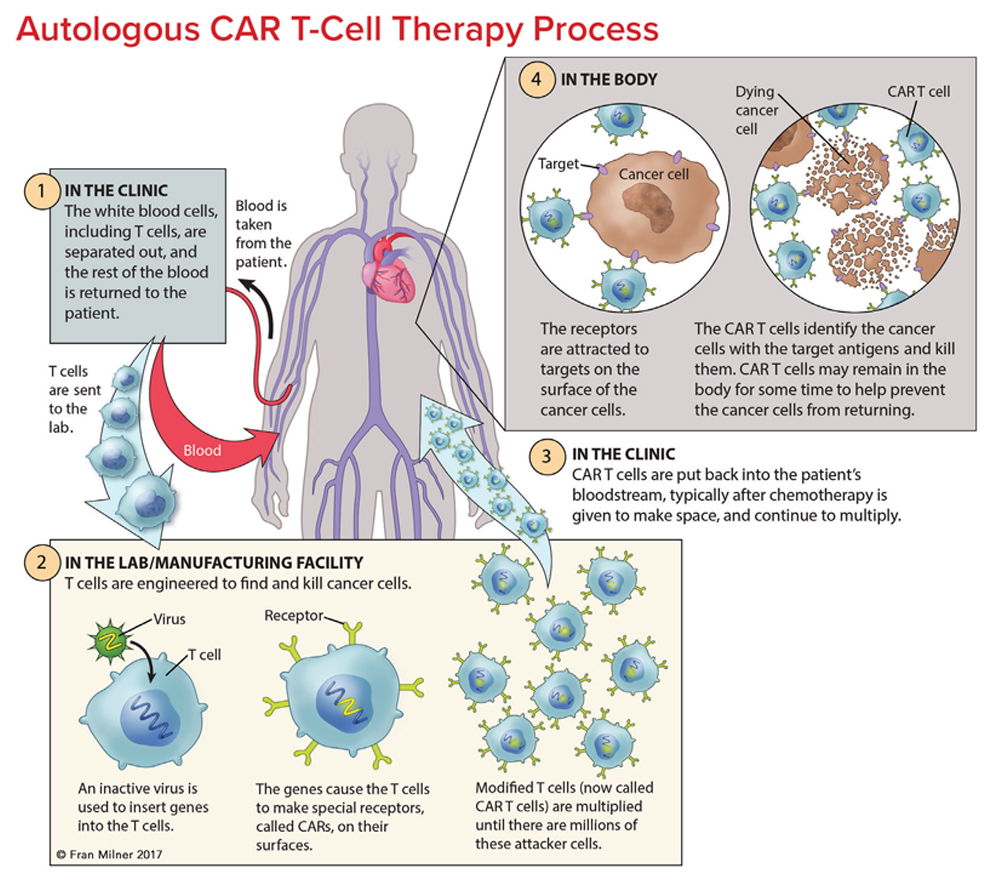
\includegraphics[width=1.0\columnwidth]{img/CART_TherapyProcess_Oct2020.jpeg}
    \end{center}
    \caption[Processo di prelievo, costituzione e somministrazione delle CAR-T]{Processo di prelievo, costituzione e somministrazione delle CAR-T
    \cite{img24}}

\end{figure}

Nonostante i risultati positivi dati dalla terapia delle CAR-T, che dimostrano il raggiungimento di risposte rapide e 
durature nel tempo, non mancano aspetti di tossicità acuta, che possono evolvere in situazioni di severità, se non 
anche di fatalità\cite{EMATOCART}.\\
La tossicità autoimmune si verifica quando il linfocita CAR-T riconosce come antigene target il CD-19 non solo nelle 
cellule cancerose, ma anche nelle cellule sane.
Il fenomeno è noto come “on-target-of-tissue effects”. È un effetto avverso che può risultare anche fatale.
È ciò che succede ai linfociti B sani, che presentano sulla loro superficie il target del linfocita CAR-T e vanno 
incontro ad aplasia. La ricerca, dovrebbe orientarsi a trovare una soluzione affinchè il target delle cellule CAR-T 
siano le cellule cancerose e non quelle sane\cite{Frontiers}.\\

Più frequentemente si assiste ad una sindrome da rilascio di citochine (CRS), che può manifestarsi con sintomi come 
astenia, febbre, mal di testa, tachicardia, ipotensione e ipossia, sintomi sistemici quali arresto cardiaco, aritmia, 
encefalopatia, insufficienza renale, fino ad arrivare ad una insufficienza multiorgano. La CRS può inoltre evolvere 
in una MAS (sindrome da attivazione macrofagica). 
La CRS può insorgere a partire da alcune ore, fino anche ad una settimana dalla somministrazione di CAR-T.\\
Diversi sono i fattori di rischio che comportano il manifestarsi di tale sintomatologia (immagine n. 25) che 
influiscono anche sul suo grado di severità; ad esempio un’ infusione di una dose elevata di CAR-T, le caratteristiche 
del paziente, il tipo di terapia di linfodeplezione, lo stato della malattia e il  burden di malattia 
(burden of disease), che dà una stima dell’impatto della malattia in termini di disabilità e mortalità\cite{EMATOCART}.\\

\begin{figure}[h]
    \begin{center}
    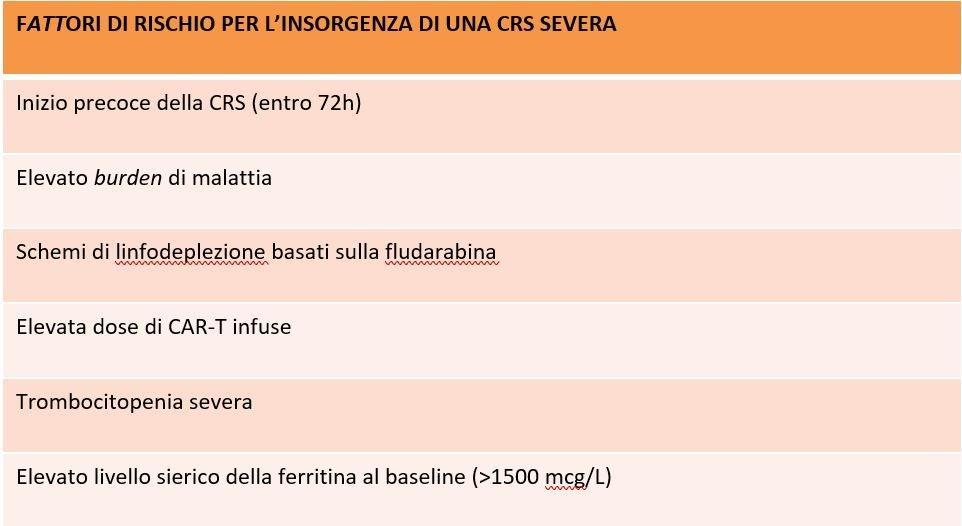
\includegraphics[width=1.0\columnwidth]{img/rischio CRS.jpeg}
    \end{center}
    \caption[Fattori di rischio per l’insorgenza di una CRS severa. ]{Fattori di rischio per l’insorgenza di una CRS severa. 
    \cite{img25}}

\end{figure}

Il grado di severità con cui si sviluppa la CRS è correlato agli elevati livelli ematici di CAR-T ed elevati livelli 
sierici di IL-6 (interleuchina-6); pertanto il trattamento di prima scelta della CRS moderata-severa, 
prevede la somministrazione di tocilizumab, un anticorpo monoclonale anti-IL-6\cite{EMATOCART}.\\
L’uso di corticosteroidi per la CRS, era precedentemente limitato, ma secondo studi più recenti il loro utilizzo 
non compromette l'attività delle CAR-T e l’outcome del paziente\cite{Cortico}.\\
Per valutare il grado di severità della CRS, l’ASTCT (American Society for Transplantation and Cellular Therapy) 
ha prodotto delle linee guida, secondo quanto riportato da \cite{ASTCT}.\\

\begin{figure}[h]
    \begin{center}
    \includegraphics[width=1.0\columnwidth]{img/severità CRS.jpeg}
    \end{center}
    \caption[Criteri di valutazione del grado di severità CRS.]{Criteri di valutazione del grado di severità CRS.
    \cite{img26}}

\end{figure}

Oltre alla CRS, la neurotossicità è un effetto collaterale comune alla terapia con CAR-T. 
L’ASTCT (American Society for Transplantation and Cellular Therapy) ha definito la neurotossicità con 
l’acronimo ICANS (Immune effector cell-associated neurotoxicity syndrome). Non sono ancora del tutto chiare le 
motivazioni per cui tale sintomatologia si presenta, sono in corso studi che cercano di spiegare i meccanismi 
fisiopatologici coinvolti.\\
L’ ICANS si manifesta con afasia, disturbi dell’attenzione, difficoltà alla scrittura, confusione, disorientamento, 
agitazione, tremori e sonnolenza. In caso di ICANS severa, i sintomi che possono presentarsi sono: crisi convulsive, 
edema cerebrale, aumento della pressione intracranica,, incontinenza, deficit di forza\cite{EMATOCART}.\\
L’ ICANS può presentarsi in concomitanza della CRS, in tal caso ha una minore durata e severità; può insorgere anche 
in seguito alla CRS con maggiore durata e severità. La durata dei sintomi è variabile, in genere è di circa 2-4 giorni,
ma può durare anche diverse settimane; i sintomi sono solitamente reversibili. 
Il trattamento terapeutico con tocilizumab è efficace in caso di ICANS associata a CRS, altrimenti la terapia di 
elezione è con corticosteroidi\cite{EMATOCART}.\\
L’ ASTCT (American Society for Transplantation and Cellular Therapy) 
ha prodotto anche per ICANS delle linee guida per valutare il grado di severità\cite{ASTCT}.\\

\begin{figure}[h]
    \begin{center}
    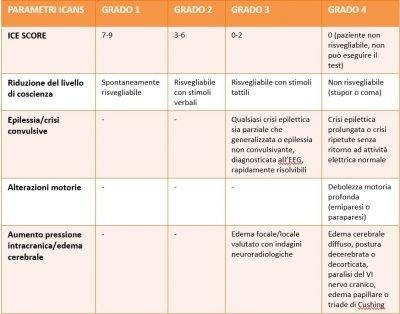
\includegraphics[width=1.0\columnwidth]{img/ICANS .jpeg}
    \end{center}
    \caption[Parametri per la valutazione del grado di severità di ICANS.]{Parametri per la valutazione del grado di severità di ICANS.
    \cite{img27}}

\end{figure}

Nella sindrome da attivazione macrofagica (MAS), si ha un’iperattività di macrofagi e linfociti, che stimolano la 
produzione di citochine pro-infiammatorie, che creano degli infiltrati tissutali, con rischio di insorgenza di 
insufficienza multiorgano.\\
I sintomi di CRS e MAS sono simili: febbre, sintomatologia neurologica, insufficienza multiorgano; 
per quanto riguarda gli esami laboratoristici si avranno livelli elevati di LDH, ferritina e citochine, mentre 
ridotti livelli di fibrinogeno\cite{EMATOCART}.
Nei pazienti in cui si sospetta una MAS, con tossicità d’organo >3, si intraprende terapia con anticorpi monoclonali 
anti-IL-6 e corticosteroidi, in caso di non miglioramento entro 48 ore, 
si prende in considerazione la terapia con etoposide.\\
La MAS refrattaria e fulminante si presenta nell’1\% circa dei pazienti trattati con CAR-T, 
se non trattata prontamente ha un’elevata mortalità\cite{EMATOCART}.\\

Una reazione anafilattica si può verificare per reazione eccessiva del sistema immunitario nei confronti del CAR, 
pertanto bisogna monitorare la comparsa di eventuali segni e sintomi coma la comparsa di eritemi, 
sudorazione, ipotensione e distress respiratorio\cite{EMATOCART}.\\
Nel caso in cui si evidenzia la comparsa di tali sintomi, il trattamento viene sospeso o terminato\cite{Frontiers}.\\

Le infezioni associate alla somministrazione di CAR-T (CTI), sono piuttosto comuni. Non è del tutto noto il meccanismo 
che le innesca e non c’è uno schema unico per la loro prevenzione e trattamento. Vi sono tuttavia una serie di fattori 
che possono indurre tali infezioni: i pazienti molto spesso sviluppano come effetto avverso alla terapia delle CAR-T 
una CRS, che può portare al ricovero del paziente in unità di terapia intensiva, dove aumenta il rischio di sviluppare 
infezioni nosocomiali; il trattamento con farmaci corticosteroidi per la CRS indebolisce il sistema immunitario; 
quest’ultimo risulta indebolito anche dalla riduzione di cellule B sane, che diventano target del CD-19 delle CAR-T; 
i pazienti che hanno un indebolimento del sistema immunitario causato dalla chemioterapia e che poi ricevono le CAR-T 
sono ad elevato rischio di sviluppare infezioni\cite{Frontiers}.\\

La Tumor Lysis Syndrome (TLS) è una complicanza abbastanza comune, maggiormente nelle neoplasie ematologiche piuttosto 
che nelle altre.\\ 
Si verifica perché un elevato numero di cellule cancerose diventano necrotiche e rilasciano i loro metaboliti e le 
loro sostanze intracellulari nel sangue; i reni non riescono ad eliminare completamente queste sostanze ed è per 
questo che si verifica la TLS.\\ 
Segni di TLS sono iperpotassiemia, iperuricemia, iperfosfatemia e ipocalcemia, in casi gravi insufficienza renale 
acuta e aritmia.\\ 
Il trattamento prevede l’ idratazione; per pazienti con rischio da basso a moderato si può intraprendere la 
somministrazione di allopurinolo in via preventiva; il rasburicase è il trattamento di elezione sia per prevenzione 
di pazienti ad alto rischio che per pazienti che hanno già sviluppato una TLS; somministrazione di diuretici e 
correzione degli squilibri idroelettrolitici\cite{Frontiers}.\\

Disturbi della coagulazione a volte si presentano, tra i 6 e i 20 giorni dopo l’infusione di CAR-T. Ci sarà un  
aumento del D-dimero, il PT allungato, trombocitopenia, diminuzione del fibrinogeno. Il rischio di CID 
(coagulazione intravascolare disseminata) è maggiore in pazienti con CRS grave, 
che risulta essere direttamente proporzionale alla gravità dei disturbi della coagulazione\cite{Frontiers}.\\

La citopenia è una reazione avversa caratterizzata da neutropenia, trombocitopenia ed anemia. 
È stato dimostrato che la citopenia che insorge in seguito alla somministrazione di CAR-T può avere una durata anche 
superiore a 30 giorni\cite{Frontiers}.\\ 
Pazienti con citopenia lieve e precoce devono avere un supporto nutrizionale e intraprendere dei trattamenti di 
prevenzione anti-infettiva.\\ 
Per pazienti con neutropenia a lungo termine, la FDA ha approvato la somministrazione mediante iniezione di Filgrastim. 
Pazienti con anemia e trombocitopenia grave vengono sottoposti a trasfusione di sangue, globuli rossi e piastrine. 
È stato anche proposto il trapianto autologo o allogenico di cellule staminali emopoietiche, come trattamento per 
la citopenia, ma la sua efficacia non è ancora ben nota\cite{Frontiers}.\\

\subsection{Immune checkpoint inhibitors}

Il sistema immunitario possiede dei checkpoint che hanno la funzione di impedire alle cellule immunitarie normali di 
attaccare le cellule sane dell’organismo. Le cellule cancerose spesso approfittano di questo meccanismo per eludere il 
sistema immunitario e sfuggire al suo controllo.\\ 
Il Pembrolizumab è un farmaco che agisce andando a bloccare questi checkpoint in modo che il sistema immunitario 
diventi responsivo verso le cellule cancerose. Tale farmaco viene usato nelle forme recidive e refrattarie di linfoma 
primitivo a cellule B del mediastino\cite{IMMUNOTP}.\\

\subsection{Immunomodulating drugs}

Si tratta di farmaci come talidomide e lenalidomide somministrati per via orale per il trattamento di alcuni tipi di 
linfoma dopo il tentativo di altri approcci terapeutici\cite{MASSIVEBIO}.\\ 
Vanno a stimolare il sistema immunitario e possono contribuire al rallentamento della crescita di cellule cancerose.\\
Sono farmaci comunque non privi di effetti collaterali, come una bassa conta di globuli bianchi, che aumenta il 
rischio di sviluppare infezioni, neuropatia, talidomide ha un maggior rischio di trombosi venosa profonda, 
fatigue e stipsi\cite{IMMUNOTP}.\\

\section{Trapianto di cellule staminali emopoietiche}

\section{Fonti di cellule staminali emopoietiche}















